\section{Sensor systems in smart environments}
In the most general definition a sensor is a device that transforms a physical property into an observable signal. This definition includes traditional systems such as mercury-based thermometers or hair-based hygrometers. Yet nowadays we are usually considering digital sensors that transfer the measured property to a binary signal that can be further processed by computing devices. 
A common variety is the smart sensor that provides additional functionality beyond generating a correct sensing signal \cite{frank2013understanding}. The main goal is to simplify installation and maintenance of distributed sensing systems by having processing close to the measurement device. Early considerations in this domain were put to the standard family IEEE 1451 - IEEE Standard for a Smart Transducer Interface for Sensors and Actuators between 1997 and 2007 \cite{ieee1451}. An additional concept is the Virtual Sensor that includes digital signal processing and conditioning and therefor abstracts the processing steps from devices interfacing the sensor. 
The number of available sensors is very high, but it is possible to restrict them based on application domain. Lewis and Cook et al. \cite{lewis2004wireless,cook2007smart} have proposed a collection for smart environments focused on wireless sensor networks. The overview is shown in table \ref{tab:sen_smart_env}.
\begin{table}[htbp]
  \centering
  \caption{Sensors for smart environments \cite{cook2007smart}}
    \begin{tabular}{rr}
    \toprule
    \textbf{Properties } & \textbf{Measurand} \\
    \midrule
    Physical properties  & Pressure, temperature, humidity, flow \\ \addlinespace
    Motion properties  & Position, velocity, angular velocity, acceleration \\ \addlinespace
    Contact properties  & Strain, force, torque, slip, vibration \\ \addlinespace
    Presence  & Tactile/contact, proximity, distance/range, motion \\ \addlinespace
    Biochemical  & Biochemical agents \\ \addlinespace
    Identification  & Personal features, RFID or personal ID \\
    \bottomrule
    \end{tabular}%

  \label{tab:sen_smart_env}%
\end{table}%
This sensor categorization is based on the property to be measured and is agnostic to the specific measurement technology. Physical properties, such as pressure, temperature, humidity and flow, can also be noted as environmental properties. They are measurements that determine the state of the smart environment, e.g. temperature in different rooms, or the current water usage. Motion properties denote the movement parameters of actors in this environment and can refer to both humans and machines. Angular velocity is important in self-localization of robots in an environment. Contact properties groups the different types of interaction between surfaces in the smart environment and actors. Presence as a group is similar to motion paramteres, but does not require a series of measurements for tracking an actor. Biochemical sensors enable measuring the presence of specifc chemical compounds in the environment and are most suited for measuring pollution or air quality. Finally, identification of actors allows to provide personalized services and can be realized with different methods ranging from tags to biometric systems.

While this listing provides a decent overview of sensing properties in smart environments it is abstracted from sensor technologies. Various types of sensors, including capacitive proximity sensors, allow us to detect multiple of these properties and thus providing a higher flexibility. Therefore it is possible to provide an inverse listing of sensor technologies that allow measuring different properties. A short overview of sensor technologies with this capabilities and that are commonly used in smart environments is given in table \ref{tab:sen_tech_prop}. In the following sections I want to give an overview on how these sensor systems are used in this domain, in order to provide a basis for the benchmarking model that will be introduced in section \ref{ch:benchmark}.
\begin{table}[htbp]
  \centering
  \caption{Sensing technologies and measured properties}
    \begin{tabular}{rr}
    \toprule
    \textbf{Technology} & \textbf{Properties} \\
    \midrule
    RGB cameras  & Motion, Presence, Identification \\ \addlinespace
    Infrared cameras & Motion, Presence, Contact \\ \addlinespace
    Ultrasound sensing & Motion, Presence, Contact, Identification \\ \addlinespace
    Microphone arrays & Motion, Presence, Contact, Identification \\ \addlinespace
    Radiofrequency sensing & Motion, Presence, Identification \\
    \bottomrule
    \end{tabular}%
  \label{tab:sen_tech_prop}%
\end{table}%

\subsection{RGB cameras}
\begin{figure}[h]
\centering
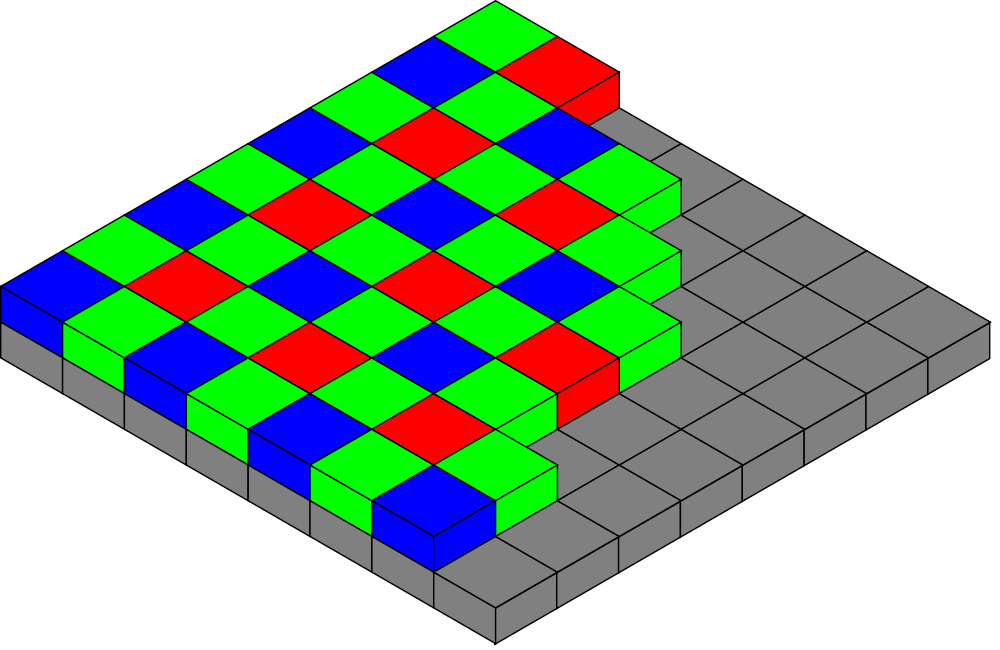
\includegraphics[width=0.4\textwidth]{images/bayer_pattern_on_sensor}
\caption{A bayer pattern on a sensor in isometric perspective \cite{img_bayer_pattern}}
\label{fig:bayer_pattern}
\end{figure}
A RGB camera is an image processing device that processes light in the visible spectrum, similar to the human eye. Modeled after the retina it has three distinct color channels - red, green and blue. There are different methods available to distinguish these channels from visible light, such as Bayer filters (Figure \ref{fig:bayer_pattern}) in front of a single sensor or using multiple sensors behind a prism.
The usage of cameras in smart environments is very common. I will present five different examples and afterwards will specify how they are linked to the properties that were defined previously.
Tabar et al. have been using a combined system of cameras, RF transmitters and wearable sensors in a home care scenario \cite{tabar2006smart}. The cameras are used to improve the accuracy of the accelerometer-based fall detection by eliminating false positives. Once a fall event occurs an algorithm tracks the posture of detected humans in the scene. They used an edge detector to distinguish the human body from other objects and applied a heuristic to differentiate lying and standing.  Additionally a face detector was used to improve the recognition of human objects. Combining this with information from the fall detecting sensor and a RF based localization system they were able to achieve a good reliability in eliminating false positive alerts.
\begin{figure}[h]
\centering
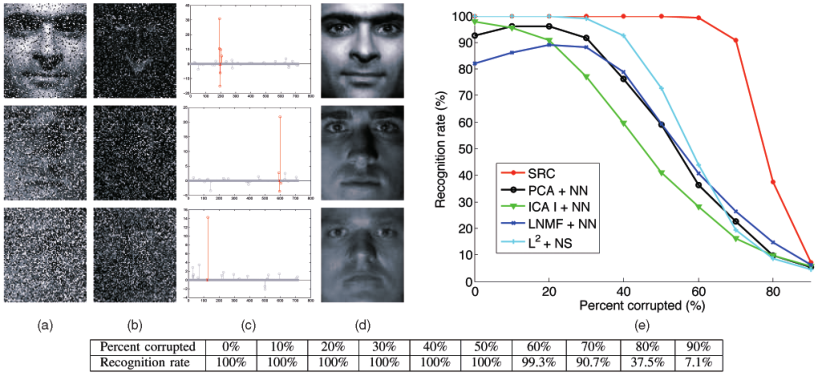
\includegraphics[width=0.9\textwidth]{images/facerec_noise}
\caption{Recognition under random corruption. (a) Top row: 30 percent of pixels are corrupted. Middle row: 50 percent corrupted. Bottom row: 70 percent corrupted. (b) Estimated errors (c) Estimated sparse coefficients (d) Reconstructed images (e) The recognition rate across the entire range of corruption for various algorithms. Newly presented (red curve) significantly outperforms others, performing almost perfectly upto 60 percent random corruption \cite{wright2009robust}}
\label{fig:facerec_noise}
\end{figure}

Pentland and Choudhury provided an overview of vision-based face recognition systems in the domain of smart environments \cite{pentland2000face}. The systems are able to identify users and recognize facial expressions. The proposed applications in smart environments include personalized shopping experiences based on customer recognition, behavior monitoring in child care facilities and emotion-aware systems that react to the user's current awareness. The described techniques include PCA-supported, eigenvector-based classification, face-based localization and systems based on local feature analysis. Newer systems are able to operate well in unconstrained environments, that include varying expression and illumination, ageing of persons, occlusion and disguise \cite{wright2009robust} (example of robustness with regard to image corruption in Figure \ref{fig:facerec_noise}).
\begin{figure}[h]
\centering
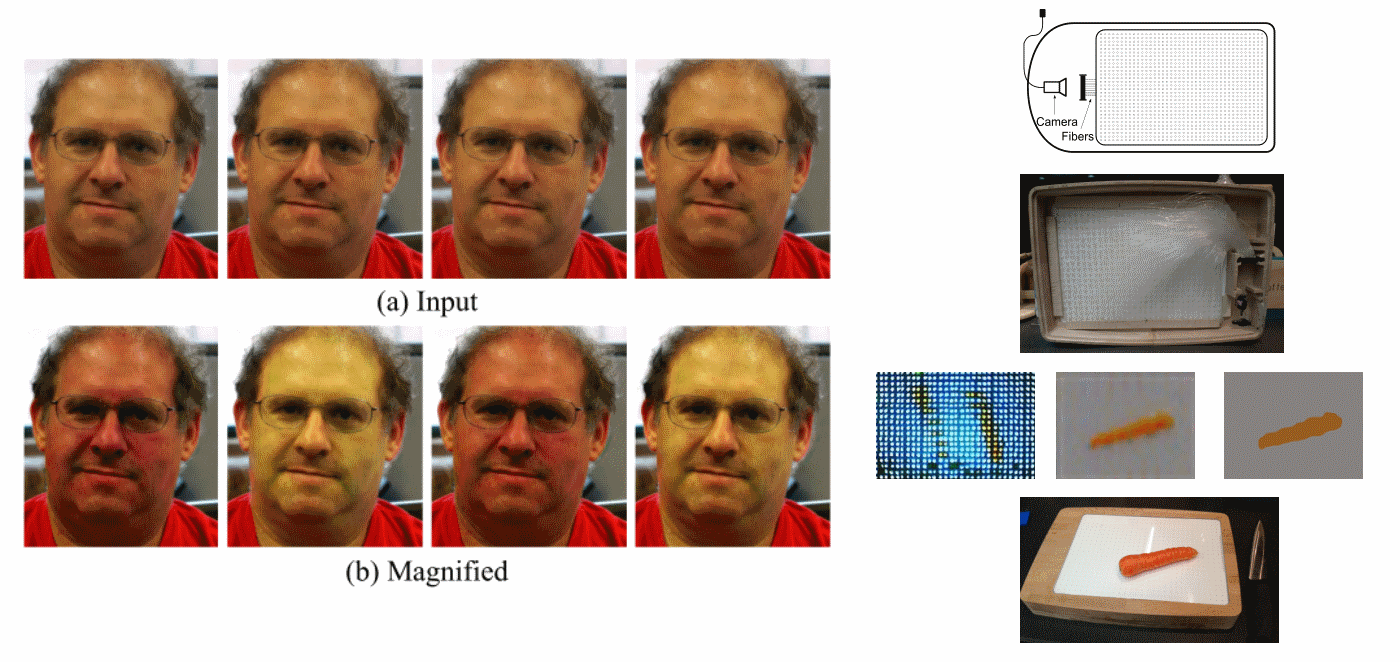
\includegraphics[width=0.7\textwidth]{images/rgb_euler_food}
\caption{\emph{Left}: Eulerian Video Magnification to attenuate the human pulse with original (a) and amplified (b) video sequence  \cite{Wu2012}. \emph{Right}: FoodBoard schematics (top), underside view (second row), original, reconstructed and segmented image (third row) and final system (bottom) \cite{pham2013foodboard}}
\label{fig:rgb_euler_food}
\end{figure}

An example for a novel image processing method that is useful in smart environments was presented by Vu et al. in 2012 \cite{Wu2012}. They are using  temporal variances of pixel values to exaggerate spatial movements and color changes that would typically be invisible to the naked eye. The method is called Eulerian Video Magnification and uses a combination of spatial decomposition and temporal filtering applied to adjacent frames. It can be tuned to different time-frequency bands to attenuate different classes of signals. Some of the proposed applications include the tracking of breathing rates of infants by attenuating chest movement, or the tracking of subtle movements, such as vibration in appliances. The example shown in Figure \ref{fig:rgb_euler_food} on the left is using a magnification of colors, in order to identify the heart rate of a person. The latter can be used for personal health applications, e.g. by integrating the system into the bath room mirror to provide an unobtrusive daily measurement and give the user feedback over a longer period of time.

A final example in this section is the FoodBoard, a smart chopping board that uses image processing to recognize the food items that are put on it \cite{pham2013foodboard}. It is shown in Figure \ref{fig:rgb_euler_food} on the right. To enable a thin footprint, ambient light is transferred to a camera using glass fibers. The picture is reconstructed and segmented, allowing to identify different items of food that are placed on it. The classification is based on a combination of Fast-Hessian and color histogram feature extractors. Pham et al. were able to distinguish 12 different ingredients with an accuracy between 59\% and 93\%. The system can be used to support dietary monitoring, give recipe guidance or support visually impaired users in identifying and tracking food.
\subsection{Infrared cameras}
Infrared imaging is using the same sensors that are suitable for visible light imaging. The difference is that they are tuned to collect electromagnetic waves of a lower wavelength that are just outside of the visible spectrum. This allows for distinct applications, such as thermal imaging, as it is possible to  detect heat radiation. In smart environments the most common application is using infrared cameras in combination with infrared light sources. This allows to illuminate spaces without visible artifacts to the user, thus providing imaging capabilities in dark rooms, or very specific conditions that may be required by a certain application. Another very interesting option is to use a specific projection of patterns into the scene. Analyzing the returning infrared light it is possible to infer the depth of specific pixels of the camera. This variety is called a depth camera. Particularly in the last few years the research in this domain has expanded strongly, sparked by the availability of an affordable depth camera/RGB camera combination - the Kinect by Microsoft \cite{zhang2012microsoft}. On the following pages we will present various examples of how this device can be used in smart environments to enable different applications in interaction and activity tracking.

\cite{beck2013immersive}

\cite{panger2012kinect}

\cite{sung2011human}

\cite{Izadi2011}
\subsection{Ultrasound sensors}
Ultrasound sensors allow detecting sound wave signals that have a frequency beyond 20kHz and are thus not audible to humans. Their propagation and reflection properties are similar to audible sound waves, thus the generated measurements can be similar. While there are natural sources of ultrasound waves the applications in smart environments do rely on active systems, that combine sound generators and sensors that measure the resulting signal. By timing the time distance between sending the signal and receiving a response it is possible to measure distances between the sender and different object. One of the earliest prototypes in Ubiquitous Computing designed by PARC was the Active Badge, an ultrasound emitter that was used to identify persons operating in the environment \cite{Weiser1991}. If various receivers are used it is possible to localize the sound source, making ultrasound sensing a popular candidate in indoor localization systems. In Figure we can see a sketch of the basic functionality of ultrasound sensing systems on the left, and an example of localization using three receivers and a single source. We will present four different examples on how ultrasound sensors are used in smart environment applications.
\cite{dutta2005utilization}

\cite{ochiai2013reflective}

\cite{watanabe2013ultrasound}

\cite{priyantha2000cricket}
\subsection{Microphone arrays}
\cite{corbishley2008breathing}

\cite{zhang2008maximum}

\cite{xu2013crowd++}

\cite{harrison2011tapsense}

\subsection{Radiofrequency sensing}
\cite{adib20133d}

\cite{wilson2010radio}

\cite{sugano2006indoor}

\cite{pu2013whole}

